\documentclass[12pt]{article}
\usepackage[spanish]{babel}
\usepackage{makeidx}
\usepackage[margin=1in]{geometry}  % set the margins to 1in on all sides
\usepackage{graphicx}              % to include figures
\usepackage{amsmath}               % great math stuff
\usepackage{amsfonts}              % for blackboard bold, etc
\usepackage{amsthm}                % better theorem environments
\usepackage{makeidx}               % index
\usepackage[utf8]{inputenc}        % now we have tildes!
\usepackage{wrapfig}               % images
\usepackage{listings}              % Unordered lists
\usepackage{hyperref}              % hyperlinks
\usepackage{xcolor}                % to colorize font
\usepackage{blindtext}             % to colorize font

\makeindex

\begin{document}

\begin{titlepage}

\newcommand{\HRule}{\rule{\linewidth}{0.5mm}} % Defines a new command for the horizontal lines, change thickness here

\center % Center everything on the page

%----------------------------------------------------------------------------------------
%	LOGO SECTION
%----------------------------------------------------------------------------------------

\textsc{\LARGE Universidad Carlos III de Madrid}\\[1.2cm] % Name of your university/college

%----------------------------------------------------------------------------------------
%	HEADING SECTIONS
%----------------------------------------------------------------------------------------


\includegraphics[width=9cm]{Logo}\\[1.2cm] % Include a department/university logo - this will require the graphicx package

\textsc{\Large Aprendizaje Automático}\\[0.5cm] % Major heading such as course name
\textsc{\large Grado en Ingeniería Informática}\\[0.6cm] % Minor heading such as course title
\textsc{\large Grupo 83}\\[0.5cm]

%----------------------------------------------------------------------------------------
%	TITLE SECTION
%----------------------------------------------------------------------------------------

\HRule \\[0.7cm]
{ \huge \bfseries Práctica 2: Aprendizaje basado en instancias}\\[0.4cm] % Title of your document
\HRule \\[0.7cm]

%----------------------------------------------------------------------------------------
%	AUTHOR SECTION
%----------------------------------------------------------------------------------------

\emph{Autores:}\\
Daniel \textsc{Medina García}\\ % Your name
Alejandro \textsc{Rodríguez Salamanca}\\[1.1cm] % Your name

%----------------------------------------------------------------------------------------
%	DATE SECTION
%----------------------------------------------------------------------------------------

{\large \today}\\ % Date, change the \today to a set date if you want to be precise

%----------------------------------------------------------------------------------------

\vfill % Fill the rest of the page with whitespace

\end{titlepage}

% TODO: a cursiva: clustering, clusters, cluster, Weka, EM, FarthestFirst, SimpleKMeans, python, i.e.

\tableofcontents

\newpage
\thispagestyle{empty}
\clearpage
\vspace*{\fill}
\begin{center}
    \begin{minipage}{\textwidth}
        \begin{center}
            \section*{Introducción}
            El presente documento contiene la memoria del trabajo realizado para esta segunda práctica de Aprendizaje Automático. En esta práctica el equipo ha utilizado el aprendizaje basado en instancias, haciendo uso de la técnica de \emph{clustering} para poder implementar funciones de afinidad y agilizar así la clasificación.

            % TODO: Revisar cuando se haya terminado porque no estoy muy seguro de lo que he puesto.
        \end{center}
    \end{minipage}
\end{center}
\vfill

\newpage
\section{Recogida de información}

% Descripción de las variables que representan el estado, así como su rango de valores.

% TODO: Depende de si tomamos o no datos nuevos, así que se queda en pendiente.

\section{Clustering}

% Descripción y justificación de los algoritmos utilizados para el proceso de clustering.

Tras probar todos los diferentes algoritmos de clustering ofrecidos por Weka, hicimos un primer filtro con aquellos que nos daban un número manejable de clusters (o se podía configurar dicho número) para evitar aquellos que generaban demasiados (menos de un 5\% de pertenencia) o insuficientes (menos de 5). Esta primera selección nos dejó con Cobweb, EM, FarthestFirst y SimpleKMeans. Comparando los algoritmos, buscamos dos propiedades: equilibrio entre los clusters y ``estabilidad" entre ejecuciones con modificamiento en los parámetros (i.e. semilla u otras constantes). Esta comparativa nos hizo decantarnos por SimpleKMeans y EM, pues los porcentajes de pertenencia a cada cluster eran más parecidos entre sí y distintas semillas resultaban en clusters de dimensiones similares.

Si bien los resultados eran parecidos entre estos dos algoritmos, el elevado coste en tiempo para elaborar el clustering con EM nos hizo decantarnos por SimpleKMeans. Mostramos a continuación la justificación de nuestra decisión, donde observamos el equilibrio conseguido con este algorimo de clustering y su estabilidad ante el cambio de la semilla. Cabe destacar que con los otros algoritmos encontramos variaciones muy superiores (e.g. 11 y 17\% con FarthestFirst, incluso 15\% con Coweb), alejadas de la media de 6\% obtenida con SimpleKMeans.

\begin{center}
    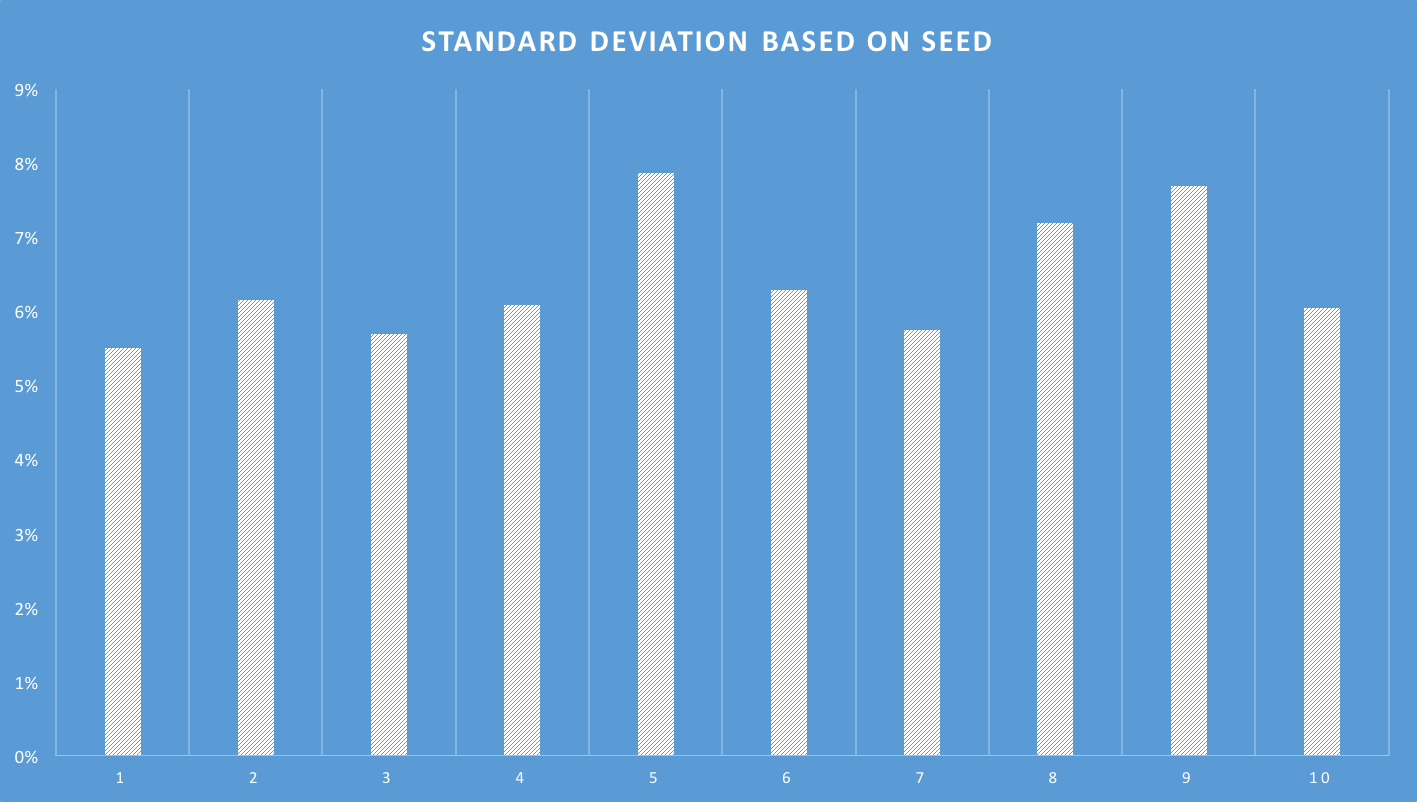
\includegraphics[width=15cm]{stdff}
\end{center}

% Descripción de cualquier tratamiento sobre los datos que se lleve a cabo y de todos los pasos realizados.

Para potenciar la eficacia de la clusterización, probamos a normalizar los datos. Sin embargo, los resultados obtenidos fueron los mismos. Como la normalización de los datos dificultaba la inclusión de nuevas instancias desde el wrapper de Weka para Python a un fichero ya normalizado, decidimos excluir este y otros filtros de preproceso de los datos. Para determinar si los movimientos tomados habían sido o no buenos, elaboramos una función cuyo incremento entre turnos supondría un rendimiento productivo. Esta función, que consta de tres sumandos con un coeficiente a modo de peso para evaluar distintos aspectos del agente, nos ayudará a descartar las instancias que no consideremos que ayuden para clusterizar correctamente.

\begin{itemize}
    \item En primer lugar, hacemos visible el acercamiento al fantasma más cercano normalizando la distancia a la que se encuentra PacMan de éste. Tomar la inversa de este dato nos asegura que un incremento en la función supone un movimiento acertado.
    \item Para evaluar el rendimiento a largo plazo, introducimos también la media de distancias normalizadas a los fantasmas. De nuevo, la inversa nos proporciona el dato que queremos incrementar.
    \item Por último, no podemos olvidarnos del objetivo principal del PacMan. Así, incluimos la cuenta de los fantasmas comidos en el último turno.
\end{itemize}

Al considerar de distinta imporancia los diferentes aspectos evaluados, incluimos los pesos de 0.5, 0.2 y 0.3 respectivamente a los sumandos previamente mencionados.

% Descripción de las estructuras de datos utilizadas para el almacenamiento de la información generada en el proceso de clustering.

Las instancias pertenecientes a cada cluster se almacenaron en un array bidimensional: la primera dimensión indica el cluster y la segunda indica el índice de cada instancia dentro del cluster. A través del wrapper clusterizamos los datos de entrada al inicializar el agente automático, y según resulten en uno u otro cluster son añadidos a un u otro array.

% Descripción de la función de pertenencia al cluster implementada.

En cuanto a la selección del cluster para cada instancia utilizamos, como anteriormente mencionamos, el algoritmo SimpleKMeans proporcionado por Weka, con 10 clusters y semilla igual a 4. El valor de la semilla es aleatorio y escogemos el cuatro como podíamos haber elegido otro, mientras que el número de clusters se ha escogido teniendo en cuenta que tenemos cuatro movimientos posibles, y varias situaciones posibles por las cuales tomar dichos movimientos, por lo que consideramos que 10 podía ser un número suficientemente significativo como para separar los datos.

\section{Generación del agente automático}

Una vez generados los clusters en los cuales separamos los datos entre los que clasificaremos las instancias nuevas, pasamos a lo que realmente integra la elección de la acción a tomar.

% Descripción de la función de similitud entre instancias implementada.

La función de similitud implementada asigna pesos a los diferentes atributos guardados de cada instancia para determinar un punto para cada instancia cuya distancia euclídea ponderada con otra instancia determinará cómo de afín le es. Repartimos los pesos según lo que consideramos ``áreas de conocimiento", o grupos de atributos que contienen una misma información. De esta forma, agrupamos la puntuación, las distancias a los fantasmas, la posición a PacMan, la dirección y la existencia de muros alrededor, quedando de la siguiente forma:
\begin{center}
    $ similarityFunc(instance) = 0.3 * livingGhosts\ +\ 0.1 * \sum\limits_{0}^{i} distanceToGhost_i\ +\ 0.2 * \sum\limits_{0}^{i} coordinate_i\ +\ 0.1 * directionValue\ +\ 0.3 * \sum\limits_{0}^{i} thereIsWall_i $
\end{center}

\newpage

\subsection{¿Por qué ha sido útil realizar clustering previa de las instancias?}

El uso de clusters permite ahorrar bastante tiempo en comparaciones para la clasificación. Al tener clusters ya hechos, sólo compararemos la instancia nueva con aquellas que pertenezcan al mismo cluster en lugar de con todo el set de entrenamiento, sabiendo que la instancia más cercana se hallará en dicho cluster.

\subsection{¿Por qué es importante usar pocos atributos en técnicas de aprendizaje no supervisado?}

% TODO Para agilizar?

\subsection{¿Qué ventaja tiene el uso del aprendizaje basado en instancias con respecto al visto en la práctica 1?}

% TODO no fucking clue, really

\subsection{¿Consideras que el agente funcionaría mejor si se introdujesen más ejemplos? ¿Por qué?}

Un conjunto de entrenamiento más grande podría ayudar a formar clusters más informados. Sin embargo, también haría más numerosas las instancias en cada cluster, ralentizando así el proceso de clasificación posterior. Este \emph{drawback} podría contrarrestarse añadiendo un mayor número de clusters.

\section{Evaluación de los agentes}

% TODO Será necesario evaluar el aprendizaje del agente automático de esta práctica. Para ello hay que realizar las siguientes tareas:

% Descripción y análisis de los resultados obtenidos en la fase de evaluación.

% 3. Evaluar para cada uno de los agentes, cómo evoluciona la distancia recorrida y enemigos muertos en cada instante de cada partida. Para ello realizar una gráfica o una tabla donde se muestre por un lado el tiempo vs distancia y otra con los fantasmas vs tiempo. Se recomienda hacer una media de todas las partidas jugadas, con lo que se realizarán dos gráficas por agente.

% 4. Una tabla resumen con las medias y desviaciones estándar de los agentes en los distintos mapas.

\newpage
\section{Conclusiones}

% TODO
% Conclusiones sobre la tarea realizada incluyendo apreciaciones m ́as generales como: para qu ́e puede ser u ́til el modelo obtenido, si al realizar la pr ́actica se os han ocurrido otros dominios en que se pueda aplicar aprendizaje autom ́atico, etc.

\vspace{0.2cm}

\centerline{\textbf{Problemas encontrados}}

\vspace{0.5cm}

% TODO

\vspace{0.5cm}

\centerline{\textbf{Comentarios personales}}

\vspace{0.5cm}

% TODO

\end{document}
